\chapter{Lineare Gleichungssysteme}
\begin{align}
	\ma{A} \cdot \vec{x} = \vec{b}, \qquad \ma{A} \in \mathbb{R}^{n\times n}; \quad \vec{b}, \vec{x} \in \mathbb{R}^n, \quad \ma{A} \neq 0\\
	\text{Theoretische: } \vec{x} = \ma{A}^{-1} \cdot \vec{b}\\
	\text{Alternativ: Lösung durch "`Division"'-Eliminierung}
\end{align}

\section{Methode zur Bestimmung von $A^{-1}$}
\begin{align}
	\ma{A}\cdot\ma{A}^{-1} &= \ma{I}\\
	\text{Sei }\ma{X} &= \ma{A}^{-1}\\
	\ma{A}\cdot\ma{X} &= \ma{I}\\
	\ma{A}\cdot\begin{bmatrix}
	\vec{x}_1 & \vec{x}_2 & \ldots & \vec{x}_n
	\end{bmatrix} &= \begin{bmatrix}
	\vec{l}_1 & \vec{l}_2 & \ldots & \vec{l}_n
	\end{bmatrix};\quad\vec{l}_1 = \begin{pmatrix}
	1\\ 0\\ \vdots\\ 0\\ 0
	\end{pmatrix}, \ldots, \vec{l}_n = \begin{pmatrix}
	0\\ 0\\ \vdots\\ 0\\ 1
	\end{pmatrix}
\end{align}
$\ma{A}\cdot\vec{x}_1 = \vec{l}_1;\quad\ma{A}\cdot\vec{x}_2 = \vec{l}_2;\quad\ldots;\ma{A}\cdot\vec{x}_n = \vec{l}_n;$\\
Nur rechte Seite ändert sich; $\ma{A} = \ma{L}\cdot\ma{U}$ nur einmal erforderlich.\\
Aufwand $n\cdot 2\cdot\frac{1}{2}(n^2 + n) = n^3 + n^2 \rightarrow O(n^3)$ für Substitution.

Probleme:
\begin{itemize}
	\item Pivot $p = 0$ \lightning\lightning
	\item Pivot $p$ "'sehr klein"'
\end{itemize}
Abhilfe: "'Pivotisierung"'- Zeilen-/Spaltentausch
\begin{itemize}
	\item "'partial pivoting"': Wähle Zeile mit betragsmäßig größtem Element in Pivotspalte
	\item "'complete pivoting"': Zeilen- und Spaltentausch
	\item Pivotisierung auch zur Aufwandreduktion (Nullelemente erhalten)
\end{itemize}

Beispiel $p = 0$
\begin{align}
	\begin{pmatrix}
	10 & -7 & 0 \\
	-3 & \num{2.1} & 6 \\
	5 & -1 & 5
	\end{pmatrix}\cdot\vec{x} &= \begin{pmatrix}
	7\\ \num{3.9}\\ 6
	\end{pmatrix}& \begin{matrix}
	p_{21} = \frac{5}{10} = \frac{1}{2}\\ p_{31} = \frac{-3}{10}
	\end{matrix}\\
	\begin{pmatrix}
	10 & -7 & 0 \\
	0 & 0 & 6 \\
	0 & \num{2.5} & 5
	\end{pmatrix}\cdot\vec{x}& = \begin{pmatrix}
	7\\ 6\\ \num{2.5}
	\end{pmatrix}& p_{32} = \frac{0}{\num{2.5}}\quad\text{\lightning}\\
	\Longrightarrow\text{ Zeilentausch}\\
	\begin{pmatrix}
	10 & -7 & 0 \\
	0 & \num{2.5} & 5 \\
	0 & 0 & 6
	\end{pmatrix}\cdot\vec{x}& = \begin{pmatrix}
	7\\ \num{2.5}\\ 6
	\end{pmatrix}
\end{align}
Zeilentausch durch Permutationsmatrix $\ma{P}$.\\
$\ma{P}\ma{A}\vec{x} = \ma{P}\vec{b}\Rightarrow$ dann $\ma{P}\ma{A}\rightarrow\ma{L}\ma{U}$\\
hier: $\ma{P} = \begin{pmatrix}
1 & 0 & 0\\ 0 & 0 & 1\\ 0 & 1 & 0
\end{pmatrix}$


\section{Kondition eines Gleichungssystems}
\begin{align}
	\begin{pmatrix}
	1 & 1\\ 1 & \num{1.0001}
	\end{pmatrix}\cdot\begin{pmatrix}
	x_1\\ x_2
	\end{pmatrix} &= \begin{pmatrix}
	2\\ 2
	\end{pmatrix}&\Rightarrow\vec{x} = \begin{pmatrix}
	2\\ 0
	\end{pmatrix}\\
	\begin{pmatrix}
	1 & 1\\ 1 & \num{1.0001}
	\end{pmatrix}\cdot\begin{pmatrix}
	x_1\\ x_2
	\end{pmatrix} &= \begin{pmatrix}
	2\\ \num{2.0001}
	\end{pmatrix}&\Rightarrow\vec{x} = \begin{pmatrix}
	1\\ 1
	\end{pmatrix}
\end{align}

Änderung in der 5. Stelle von $\vec{b}$ wird zu einer Änderung in der ersten Stelle der Lösung $\vec{x}$ "'verstärkt"'. System reagiert sehr sensitiv auf kleine Änderungen der Ausgangsdaten. Kein Lösungsalgorithmus kann etwas daran ändern.
\begin{align}
	\cond{\ma{A}} = \num{4.0002e4}
\end{align}

\section{Einfluss der Pivotisierung auf die Ergebnisgenauigkeit}
\begin{align}
	\ma{B}\rightarrow\begin{pmatrix}
	\num{0.0001} & 1 \\ 1 & 1
	\end{pmatrix}\cdot\vec{x} &= \begin{pmatrix}
	1\\ 2
	\end{pmatrix}\\
	\begin{pmatrix}
	\num{0.0001} & 1 \\ 0 & -9999
	\end{pmatrix}\cdot\vec{x} &= \begin{pmatrix}
	1\\ -9998
	\end{pmatrix}\quad\Rightarrow\begin{matrix}
	x_2 = \num{0.99989998}\\ x_1 = \num{1.00010001}
	\end{matrix}
\end{align}

Annahme: 3 Stellen Genauigkeit
\begin{align}
	\begin{pmatrix}
	\num{0.0001} & 1 \\ 0 & -\num{10000}
	\end{pmatrix}\cdot\vec{x} = \begin{pmatrix}
	1\\ -\num{10000}
	\end{pmatrix}\quad\Rightarrow\begin{array}{l}
	x_2 = 1\\ x_1 = 0\text{ \lightning}
	\end{array}
\end{align}

Zerlegung $\ma{B} = \ma{L}\ma{D}\ma{U}$ (ohne Genauigkeitsbeschränkung)
\begin{align}
	\begin{array}{c}
	\text{("'out of}\\ \text{scale}\\ \text{with }\ma{B}\text{ "')}
	\end{array}\quad = \begin{pmatrix}
	1 & 0 \\
	\num{10000} & 1
	\end{pmatrix}\cdot\begin{pmatrix}
	\num{0.0001} & 0 \\ 0 & -9999
	\end{pmatrix}\cdot\begin{pmatrix}
	1 & \num{10000} \\
	0 & 1
	\end{pmatrix}
\end{align}

Änderung der Pivotisierungsreihenfolge
\begin{align}
	\begin{pmatrix}
	1 & 1 \\ \num{0.0001} & 1
	\end{pmatrix}\cdot\vec{x} &= \begin{pmatrix}
	2\\ 1
	\end{pmatrix}\\
	\begin{pmatrix}
	1 & 1 \\ 0 & \num{0.9999}
	\end{pmatrix}\cdot\vec{x} &= \begin{pmatrix}
	2\\ \num{0.9998}
	\end{pmatrix}\quad\Rightarrow\begin{matrix}
	x_2 = \num{0.99989998}\\ x_1 = \num{1.00010001}
	\end{matrix}
\end{align}

Annahme: 3 Stellen Genauigkeit
\begin{align}
	\begin{pmatrix}
	1 & 1 \\ 0 & 1
	\end{pmatrix}\cdot\vec{x} &= \begin{pmatrix}
	2\\ 1
	\end{pmatrix}\quad\Rightarrow\begin{rcases}
	x_2 = 1\\ x_1 = 0
	\end{rcases}\quad\begin{matrix}
	\text{nur sehr geringer}\\ \text{Genauigkeitsverlust}
	\end{matrix}
\end{align}
NB: $\cond{\ma{B}} = \num{2.61838527}$

Uns interessieren also zwei Themen:
\begin{itemize}
	\item \textbf{Kondition} der Gleichungssystems
	\item \textbf{Stabilität} des Lösungsverfahrens
\end{itemize}

\section{Kondition einer Matrix}
Ausgehend von einem linearen Gleichungssystem
\[\ma{A} \cdot \vec{x} = \vec{b}\]
kann man auf der rechten Seite einen Fehler $\Delta \vec{b}$ hinzufügen.
\[\ma{A} \left( \vec{x} + \Delta \vec{x} \right) = \vec{b} + \Delta \vec{b}\]
Dieser resultiert dann in einem Fehler $\Delta \vec{x}$ der Lösung in $\vec{x}$.
Der Zusammenhang zwischen diesen Größen lautet
\[\ma{A} \Delta \vec{x} = \Delta \vec{b}\]
und kann umgeformt werden zu
\[ \Delta \vec{x} = \ma{A}^{-1} \Delta \vec{b}\]
\[ ||\Delta \vec{x}|| \le ||\ma{A}^{-1}|| \cdot ||\Delta \vec{b}||\]
Gleichzeitig kann
\[\vec{b} = \ma{A} \vec{x}\]
umgeformt werden zu
\[||\vec{b}|| \le ||\ma{A}|| \cdot ||\vec{x}||\]
\[\frac{1}{||\vec{x}||} \le ||\ma{A}|| \cdot \frac{1}{||\vec{b}||}\]
Diese Gleichungen zusammengefasst ergeben dann
\[\frac{||\Delta \vec{x}||}{||\vec{x}||} \le ||\ma{A}^{-1}|| \cdot ||\ma{A}|| \cdot \frac{||\Delta \vec{b}||}{||\vec{b}||}\]
Darin stellen dann $\frac{||\Delta \vec{x}||}{||\vec{x}||}$ den relativen Fehler des Ergebnisses, $||\ma{A}^{-1}|| \cdot ||\ma{A}||$ den \emph{Verstärkungsfaktor} für Fehler in $\vec{b}$ und $\frac{||\Delta \vec{b}||}{||\vec{b}||}$ den relativen Fehler in $\vec{b}$ dar. Wir definieren die Kondition von A über
\[\cond{\ma{A}} = ||\ma{A}^{-1}|| \cdot ||\ma{A}||\]
welche offensichtlich abhängig von der gewählten Matrixnorm ist. Eine $\cond{\ma{A}} \rightarrow \infty$ bedeutet dabei eine schlechte, $\cond{\ma{A}} \rightarrow 0$ eine gute \emph{Kondition}.

\section{Allgemeines Iterationsverfahren für lineare Gleichungssysteme}
\begin{align}
	\ma{A} \cdot \vec{x} &= \vec{b}\\
	\vec{x}^{(k+1)} &= \vec{\Phi} \left( \vec{x}^{(k)}\right)\\
	\ma{B} &\text{ beliebig}\\
	\ma{B} \vec{x} + \left( \ma{A} - \ma{B} \right) \vec{x} &= \vec{b} \quad \\
	\Rightarrow \text{ Iterationsvorschrift:}&\\
	\ma{B} \cdot \vec{x}^{(k+1)} + \left(  \ma{A} - \ma{B} \right) \cdot \vec{x}^{(k)} &= \vec{b}\\
	\vec{x}^{(k+1)} &= \vec{x}^{(k)} - \ma{B}^{-1} \cdot \left( \ma{A} \cdot \vec{x}^{(k)} - \vec{b} \right) \\
	&= \underbrace{\left( \ma{I} - \ma{B}^{-1} \cdot \ma{A}\right)}_{\text{Konvergenz, wenn }|\lambda| < 1} \cdot \vec{x}^{(k)} + \ma{B}^{-1} \cdot \vec{b}
\end{align}

\subsection{Iterative Verfahren zum Lösen linearer Gleichungssysteme}
\[\ma{A} \vec{x} = \vec{b},\ \ma{A} \in \mathrm{R}^{n\times n},\ \vec{x},\vec{b} \in \mathrm{R}^n,\ \ma{A} \text{ nicht singulär}\]

\begin{align}
	\textbf{Splitting: } \ma{A} &= \begin{bmatrix}a_{ij}\end{bmatrix} = \ma{D} + \ma{L} + \ma{U}\\
	&= \begin{bmatrix}a_{11} & & & \\ & a_{22} & &\\ & & \ddots & \\ & & & a_{nn}\end{bmatrix} +
	\begin{bmatrix}0 & & & \\ a_{21} & 0 & &\\ \vdots & & \ddots &  \\ a_{n1} & \ldots & a_{n\, n-1} & 0\end{bmatrix} +
	\begin{bmatrix}0 & a_{12} & \ldots & a_{1n} \\ & 0 & & \vdots \\ & & \ddots & a_{n-1\,n} \\ & & & 0\end{bmatrix}
\end{align}

\begin{align}
	\ma{A} &= \ma{S} - \ma{T}\\
	\ma{A} \cdot \vec{x} &= \left( \ma{S} - \ma{T} \right) \cdot \vec{x} = \vec{b}\\
	\Rightarrow \ma{S} \cdot \vec{x} &= \ma{T} \cdot \vec{x} + \vec{b}\\
	&= \left( \ma{S} - \ma{A} \right) \cdot \vec{x} + \vec{b}\\
	\Rightarrow \vec{x} &= \ma{S}^{-1} \cdot \left( \ma{S} - \ma{A} \right) \cdot \vec{x} + \ma{S}^{-1} \cdot \vec{b}
\end{align}

\ldots

\subsection{Verschiedene Iterationsverfahren}
\begin{enumerate}
	\item $\ma{S} = \ma{D}\quad$ : Jacobi (Gesamtschrittverfahren)
	\item $\ma{S} = \ma{D}+\ma{L}\quad$ : Gauß-Seidl (Einzelschrittverfahren)
	\item $\ma{S} = \frac{1}{w}(\ma{D}+w\ma{L})\quad$ : sukzessive Überrelaxation (SOR, successive Over-Relaxation)
\end{enumerate}
\begin{enumerate}
	\item Jacobi: $\ma{S} = \ma{D};\ma{D}$ nicht singulär (d.h. $a_{ii}\neq 0$)
	\begin{align}
		{A}\vec{x} = \vec{b}\Rightarrow\ma{D}\cdot\vec{x}^{(k+1)} &= (\ma{D}-\ma{A})\cdot\vec{x}^{(k)}+\vec{b} = (-\ma{L}-\ma{U})\cdot\vec{x}^{(k)}+\vec{b}\\
		\vec{x}^{(k+1)} &= \underbrace{\ma{D}^{-1}\cdot(-\ma{L}-\ma{U})}_{\ma{K}_j}\cdot\vec{x}^{(k)}+\underbrace{\ma{D}^{-1}\vec{b}}_{\vec{c}_j}\\
		&= \ma{K}_j\cdot\vec{x}^{(k)}+\vec{c}_j
	\end{align}
	\item Gauss-Seidel: $\ma{S} = \ma{D} + \ma{L}$ (nicht singulär)
	\[\ma{A} \vec{x} + \vec{b} = \vec{0} \Rightarrow (\ma{D} + \ma{L}) \vec{x}^{(k + 1)} = (\ma{D} + \ma{L} - \ma{A}) \vec{x}^{(k)} + \vec{b} = -\ma{U} \vec{x}^{(k)} + \vec{b}\]
	\[\vec{x}^{(k + 1)} = \underbrace{-(\ma{D} + \ma{L})^{-1} \cdot \ma{U}}_{\ma{K}_g} \vec{x}^{(k)} + \underbrace{(\ma{D} + \ma{L})^{-1} \vec{b}}_{\vec{c}_g}\]
	\[\vec{x}^{(k + 1)} = \ma{K}_g \vec{x}^{(k)} + \vec{c}_g\]
	\item Successive Over-Relaxation: $\ma{S} = \frac{1}{\omega} (\ma{D} + \omega \ma{L})$
	\[\ma{A} \vec{x} = \vec{b}\]
	\[\frac{1}{\omega} (\ma{D} + \omega \ma{L}) \vec{x}^{(k + 1)} = \frac{1}{\omega} (\ma{D} + \omega \ma{L} - \omega \ma{A}) \vec{x}^{(k)} + \vec{b}\]
	\[\left( \ma{D} + \omega \ma{L} \right) \vec{x}^{(k + 1)} = (\ma{D} + \omega \ma{L} - \omega \ma{A}) \vec{x}^{(k)} + \omega \vec{b}\]
	\[\left( \ma{D} + \omega \ma{L} \right) \vec{x}^{(k + 1)} = (\ma{D}(1 - \omega) - \omega \ma{U}) \vec{x}^{(k)} + \omega \vec{b}\]
	\[\vec{x}^{(k + 1)} = \underbrace{(\ma{D} + \omega \ma{L})^{-1} (\ma{D} (1 - \omega) - \omega \ma{U})}_{\ma{K}_\omega} \vec{x}^{(k)} + \underbrace{\left( \ma{D} + \omega \ma{L} \right)^{-1} \omega \vec{b}}_{\vec{c}_\omega}\]
	\[\vec{x}^{(k + 1)} = \ma{K}_\omega \vec{x}^{(k)} + \vec{c}_\omega\]
	Die jeweilige Wahl von $\omega$ bei SOR beeinflusst dann das Konvergenzverhalten. Für Spezialfälle können Empfehlungen gegeben werden:
	\begin{enumerate}
		\item Falls $a_{ii} \ne 0$, $i = 1, \dots, n$ $\Rightarrow \varrho(\ma{K}_\omega) \ge |1 - \omega| \Rightarrow$ Konvergenz für $0 < \omega < 2$
		\item Falls $\ma{A}$ positiv definit und $0 < \omega < 2$, dann konvergiert SOR für jede Initiallösung $\vec{x}^{(0)}$
		\item Falls $\ma{A}$ positiv definit und tridiagonal ist, dann $\varrho(\ma{K}_g) = \varrho(\ma{K}_j)^2 < 1$ und die optimale Wahl für $\omega$ ist:
		\[\omega = \frac{2}{1 + \sqrt{1 - \varrho(\ma{K}_j)^2}}\]
	\end{enumerate}
\end{enumerate}
Ein Beispiel zum Vergleich zwischen Jacobi und Gauß-Seidel
\begin{align}
10 x_1 - x_2 + 2 x_3 &= 6 \\
- x_1 + 11 x_2 - x_3 + 3 x_4 &= 25 \\
2 x_1 - x_2 + 10 x_3 - x_4 &= -11 \\
3 x_2 - x_3 + 8 x_4 &= 15
\end{align}

Jacobi:
\begin{align}
	x_1^{(k + 1)} &= \frac{1}{10} x_2^{(k)} - \frac{1}{5} x_3^{(k)} + \frac{3}{5} \\
	x_2^{(k + 1)} &= \frac{1}{11} x_1^{(k)} + \frac{1}{11} x_3^{(k)} - \frac{3}{11} x_4^{(k)} + \frac{25}{11} \\
	x_3^{(k + 1)} &=  -\frac{1}{5} x_1^{(k)} + \frac{1}{10} x_2^{(k)} + \frac{1}{10} x_4^{(k)} - \frac{11}{10} \\
	x_4^{(k + 1)} &= -\frac{3}{8} x_2^{(k)} + \frac{1}{8} x_3^{(k)} + \frac{15}{8}
\end{align}

Gauß-Seidel:
\begin{align}
x_1^{(k + 1)} &= \frac{1}{10} x_2^{(k)} - \frac{1}{5} x_3^{(k)} + \frac{3}{5} \\
x_2^{(k + 1)} &= \frac{1}{11} x_1^{(k + 1)} + \frac{1}{11} x_3^{(k)} - \frac{3}{11} x_4^{(k)} + \frac{25}{11} \\
x_3^{(k + 1)} &= -\frac{1}{5} x_1^{(k + 1)} + \frac{1}{10} x_2^{(k + 1)} + \frac{1}{10} x_4^{(k)} - \frac{11}{10} \\
x_4^{(k + 1)} &= -\frac{3}{8} x_2^{(k + 1)} + \frac{1}{8} x_3^{(k + 1)} + \frac{15}{8}
\end{align}
Man erkennt bei Gauß-Seidel die Abhängigkeit von Werten, welche erst im aktuellen Iterationsschritt berechnet werden. In der Praxis bietet Gauß-Seidel dadurch in der Regel eine schneller Konvergenz. Vorteil von Jacobi ist jedoch die bessere Parallelisierbarkeit eines Iterationsschrittes.

\subsubsection{Konvergenzbetrachtung}
\begin{equation}
	\ma{S} \vec{x} = \ma{T} \vec{x} + \vec{b}
	\label{eq:jacobi_konvergenz_1}
\end{equation}
\begin{equation}
	\ma{S} \vec{x}^{(x + 1)} = \ma{T} \vec{x}^{(k)} + \vec{b}
	\label{eq:jacobi_konvergenz_2}
\end{equation}

\ref{eq:jacobi_konvergenz_1} - \ref{eq:jacobi_konvergenz_2}:
\[\ma{S} (\vec{x} - \vec{x}^{(k + 1)}) = \vec{T} (\vec{x} - \vec{x}^{(k)})\]
\[\ma{S} \vec{e}^{(k + 1)} = \ma{T} \vec{e}^{(k)}\]
\[\vec{e}^{(k + 1)} = \ma{S}^{-1} \ma{T} \vec{e}^{(k)}\]
\[\vec{e}^{(k + 1)} = \ma{G} \vec{e}^{(k)} = \ma{G}^k \vec{e}^{(0)}\]

\subsection{Gradientenverfahren}
Sei $ \ma{A} \in \mathbb{R}^{n\times n} $ mit
\begin{itemize}
	\item $\ma{A}^T = \ma{A}$
	\item $\vec{x}^T \cdot \ma{A} \cdot \vec{x} > 0$ für $\vec{x} \neq 0$ (positiv definit)
	\item $\vec{b} \in \mathbb{R}$
\end{itemize}

Dann existiert genau ein Minimum für die quadratische Form:
\begin{align}
	\Phi(\vec{x}) &= \num{0.5} \cdot \vec{x}^T \cdot \ma{A} \cdot \vec{x} - \vec{x}^T \cdot \vec{b}\\
	\nabla \Phi(\vec{x}) &= \num{0.5} \left( \ma{A}^T + \ma{A} \right) \cdot \vec{x} - \vec{b} = \ma{A} \cdot \vec{x} - \vec{b}\\
	\text{Minimum: } \nabla \Phi(\vec{x}) = \vec{0} \Rightarrow \ma{A} \cdot \vec{x} = \vec{b}
\end{align}

$\Rightarrow$ Minimierung der quadratischen Form entspricht Lösung des linearen Gleichungssystem.

\section{Iterativer Ansatz für Minimierungsproblem}
\begin{tabular}{ll}
	\textbf{Allgemein:} & $\vec{x}^{(k+1)} = \vec{x}^{(k)} + \alpha_K \cdot \vec{d}^{(k)}$\\
	\textbf{Bestimme:} & $\alpha_k,\ \vec{d} = ?$\\
	\textbf{Idee:} & Wähle Richtung des steilsten Abstiegs ("'steepest descent"', siehe \autoref{fig:steepest-descent})\\
\end{tabular}

\begin{figure}
	\center
	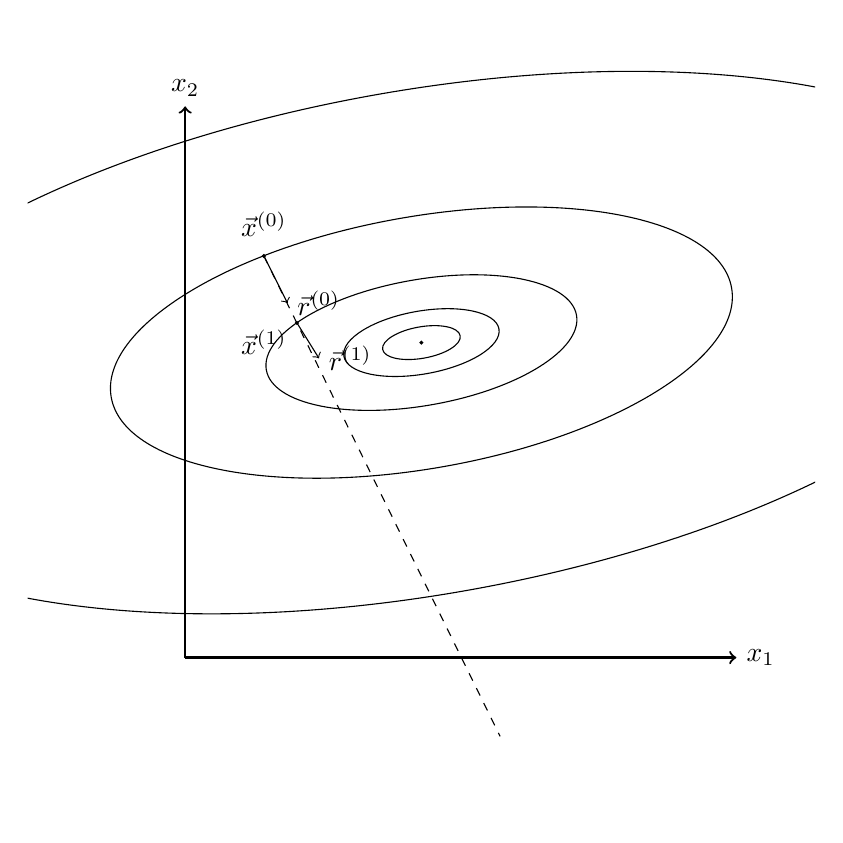
\begin{tikzpicture}	
	\coordinate (center) at (3, 4);
	
	\clip (-2, -2) -- (8, -2) -- (8, 8) -- (-2, 8) -- (-2, -2);
	\draw[thick,->] (0,0) -- (7,0) node[right]{$x_1$};
	\draw[thick,->] (0,0) -- (0,7) node[above]{$x_2$};
	\node[draw,circle,inner sep=0.2pt,fill,black] at (center) {};
	\draw[rotate=10] (center) ellipse (0.5cm and 0.2cm);
	\draw[rotate=10] (center) ellipse (1cm and 0.4cm);
	\draw[rotate=10] (center) ellipse (2cm and 0.8cm);
	\draw[rotate=10] (center) ellipse (4cm and 1.6cm);
	\draw[rotate=10] (center) ellipse (8cm and 3.2cm);
	
	\node[draw,circle,inner sep=0.2pt,fill,black] at (1, 5.1) {};
	\node at (1, 5.5) {$\vec{x}^{(0)}$};
	\draw[->] (1, 5.1) -- (1.3, 4.5) node[right] {$\vec{r}^{(0)}$};
	\draw[thin, dashed] (1, 5.1) -- (4, -1) node[right] {};
	\node[draw,circle,inner sep=0.2pt,fill,black] at (1.42, 4.25) {};
	\node at (1, 4) {$\vec{x}^{(1)}$};
	\draw[->] (1.42, 4.25) -- (1.7, 3.8) node[right] {$\vec{r}^{(1)}$};

\end{tikzpicture} 

	\caption{Gradientenverfahren - steepest descent}
	\label{fig:steepest-descent}
\end{figure}

\begin{align}
	\vec{d}^{(k)} &= - \nabla \Phi(\vec{x}^{(k)}) = \vec{b} - \ma{A} \vec{x}^{(k)} =: \vec{r}^{(k)} \text{ Residium}\\
\end{align}
$\alpha_k = ? \quad \Rightarrow $ Minimiere $ \vec{\Phi}$\\
\begin{align}
	\vec{x}^{(k+1)} &= \vec{x}^{(k)} + \alpha_k \vec{r}^{(k)}\\
	\vec{\Phi}(x^{(k+1)}) &= \frac{1}{2} \left( \vec{x}^{(k)} + \alpha_k \vec{r}^{(k)}\right)^T \cdot \ma{A} \cdot \left( \vec{x}^{(k)} + \alpha_k \vec{r}^{(k)}\right) - \left( \vec{x}^{(k)} + \alpha_k \vec{r}^{(k)}\right)^T \cdot \vec{b}\\
	\frac{\partial \vec{\Phi}(x^{(k+1)})}{\partial \alpha_k} &= \frac{1}{2} \vec{r}^{{(k)}^T} \cdot \ma{A} \cdot \vec{x}^{(k)} + \frac{1}{2} \vec{x}^{{(k)}^T} \cdot \ma{A} \cdot \vec{r}^{(k)} + \alpha_k \cdot \vec{r}^{{(k)}^T} \cdot \ma{A} \cdot \vec{r}^{(k)} - \vec{r}^{{(k)}^T} \cdot \vec{b}\\
	&= \vec{r}^{{(k)}^T} \cdot \ma{A} \vec{x}^{(k)} - \vec{r}^{{(k)}^T} \cdot \vec{b} + \alpha_k \cdot \vec{r}^{{(k)}^T} \cdot \ma{A} \cdot \vec{r}^{(k)} \neq 0\\
	\ldots\\
	\Rightarrow \alpha_k &= \frac{\vec{r}^{{(k)}^T} \cdot \vec{r}^{(k)}}{\vec{r}^{{(k)}^T} \cdot \ma{A} \cdot \vec{r}^{(k)}}
\end{align}
\textbf{Verfahren: }\\
Für $k = 0,1,2,\ldots$
\begin{align}
	\vec{r}^{(k)} &= \vec{b} - \ma{A} \vec{x}^{(k)}\\
	\alpha_k &= \frac{\vec{r}^{{(k)}^T} \cdot \vec{r}^{(k)}}{\vec{r}^{{(k)}^T} \cdot \ma{A} \cdot \vec{r}^{(k)}}\\
	\vec{x}^{(k+1)} &= \vec{x}^{(k)} + \alpha_k \cdot \vec{r}^{(k)} \label{eq:verfahren-schritt-3}
\end{align}

2 Matrix-Vektormultiplikationen (dominant)\\
2 Vektor-Skalarprodukte\\
\textbf{Alternative:}
\begin{align}
	- \ma{A} \cdot \vec{x}^{(k+1)} + \vec{b} &= - \ma{A} \cdot \vec{x}^{(k)} - \alpha_k \cdot \ma{A} \cdot \vec{r}^{(k)} + \vec{b}\\
	\vec{r}^{(k+1)} &= \vec{r}^{(k)} - \alpha_k \cdot \ma{A} \vec{r}^{(k)}
\end{align}
$\Rightarrow$ \text{ nur eine Matrix-Vektormultiplikation je Iteration}

\subsection{Konvergenz}
\begin{align}
	\vec{x}^{(k)} &= \vec{x}^* + \vec{e}^{(k)} \text{, Annahme: } \vec{e} \text{ is EV von } \ma{A}:\\
	\ma{A} \cdot \vec{e} &= \lambda_e \cdot \vec{e}\\
	\vec{r}^{(k)} &= \vec{b} - \ma{A} \cdot \vec{x}^{(k)}\\
	&= \vec{b} - \ma{A} \cdot \left( \vec{x}^* + \vec{e}^{(k)}\right)\\
	&= \underbrace{\vec{b} - \ma{A} \cdot \vec{x}^*}_{\vec{0}} - \ma{A} \cdot \vec{e}^{(k)}\\
	\vec{r}^{(k)} &= - \ma{A} \cdot \vec{e}^{(k)} = - \lambda_e \cdot \vec{e}^{(k)} \Rightarrow \vec{r}^{(k)} \text{ ist ebenfalls EV}
\end{align}

\begin{align}
	\text{Aus \autoref{eq:verfahren-schritt-3}: } \vec{x}^{(k+1)} &= \vec{x}^{(k)} + \alpha_k \cdot \vec{r}^{(k)}\\
	\vec{e}^{(k+1)} &= \vec{e}^{(k)} + \alpha_k \cdot \vec{r}^{(k)}\\
	&= \vec{e}^{(k)} + \frac{\vec{r}^{{(k)}^T} \cdot \vec{r}^{(k)}}{\vec{r}^{{(k)}^T} \cdot \ma{A} \cdot \vec{r}^{(k)}} \cdot \left( -\lambda_e \cdot \vec{e}^{(k)}\right)\\
	&= \vec{e}^{(k)} + \frac{\vec{r}^{{(k)}^T} \cdot \vec{r}^{(k)}}{\vec{r}^{{(k)}^T} \cdot \vec{r}^{(k)} \cdot \lambda_e} \cdot \left( -\lambda_e \cdot \vec{e}^{(k)}\right)\\
	&= \vec{e}^{(k)} - \vec{e}^{(k)} = \vec{0} \Rightarrow \text{Exakte Lösung in einem Schritt}
\end{align}

\textbf{Allgemein}

\begin{align}
||\vec{x}||_A &= \sqrt{\vec{x}^T \cdot \ma{A} \cdot \vec{x}} \text{ Energienorm}\\
\text{Es gilt: } ||\vec{e}^{(k+1)}||_A &= \frac{\kappa_2(\ma{A})-1}{\kappa_2(\ma{A})+1} \cdot ||\vec{e}^{(k)}||_A
\end{align}
mit $\kappa_2$ als die Kondition bezüglich der Spektralnorm

\section{CG - Konjugierte Gradientenmethode}
$ \vec{p}^{(k)} $ ist eine Menge mit $ \underbrace{\vec{p}^{{(i)}^T}}_{\text{paarweise A-orthogonal bzw. A-konjugiert}} \cdot \ma{A} \cdot \vec{p}^{(j)} = 0, \forall i,j=1,\ldots,n\quad i \neq j$\\
$ \Rightarrow \vec{p}^{(k)}$ bilden eine Basis des $\mathbb{R}^n$

\begin{align}
\text{Daher: } \vec{x}^* &= \sum^n_{i=1} \alpha_i \cdot \vec{p}^{(i)}\\
\Rightarrow \vec{b} &= \ma{A} \cdot \vec{x}^* = \sum^n_{i=1} \alpha_i \cdot \ma{A} \cdot \vec{p}^{(i)}
\end{align}

\subsection{Schrittweite}
\begin{align}
0 = \frac{\partial\vec{\Phi}}{\partial\alpha_k}\left(\vec{x}^{(k)}+\alpha_k\vec{p}^{(k)}\right)\\
\Rightarrow\alpha_k = \frac{\vec{p}^{{(k)}^T}\cdot\vec{r}^{(k)}}{\vec{p}^{{(k)}^T}\cdot\ma{A}\cdot\vec{p}^{(k)}}
\end{align}
Wie Gradientenverfahren, aber Suchrichtung $\vec{p}$

\subsection{Suchrichtung}
\textbf{Definition:} Lösung $\vec{x}^{(k)}$ heißt optimal bzgl. einer Richtung $\vec{p}\neq 0$, wenn $\vec{\Phi}(\vec{x}^{(k)})\leq\vec{\Phi}(\vec{x}^{(k)}+\lambda\vec{p})\;,\;\forall\lambda\in\R$\\
\begin{itemize}
\item[$\Leftrightarrow$] $\vec{\Phi}$ besitzt lokales Minimum entlang $\vec{p}$ für $\lambda = 0$
\item[$\Leftrightarrow$] $\frac{\partial\vec{\Phi}}{\partial\lambda}\left(\vec{x}^{(k)}+\lambda\vec{p}^{(k)}\right)\vert_{\lambda = 0} = \vec{p}^T\cdot\ma{A}\cdot\vec{x}^{(k)} - \vec{p}\vec{b}^T + \lambda\vec{p}^T\cdot\ma{A}\cdot\vec{p}\vert_{\lambda = 0}$
\item[$\Leftrightarrow$] $\vec{p}\vec{I}\vec{r}^{(k)}$
\end{itemize}
\begin{align}
\text{Sei }\vec{x}^{(k+1)} = \vec{x}^{(k)} + \vec{q}\Rightarrow\vec{r}^{(k+1)} &= \vec{b}\cdot\ma{A}\cdot\vec{x}^{(k+1)}\\
&= \vec{b}\cdot\ma{A}\cdot\vec{x}^{(k)} - \ma{A}\vec{q}\\
&= \vec{r}^{(k)} - \ma{A}\vec{q}
\end{align}
Forderung $\vec{x}^{(k+1)}$ ebenfalls optimal bzgl. $\vec{p}$, also
\begin{align}
0 = \vec{p}^T\cdot\vec{r}^{(k+1)} &= \vec{p}^T\cdot(\vec{r}^{(k)} - \ma{A}\vec{q})\\
&= \underbrace{\vec{p}^T\cdot\vec{r}^{(k)}}_{0}-\vec{p}^T\cdot\ma{A}\cdot\vec{q} = \underbrace{-\vec{p}^T\cdot\ma{A}\cdot\vec{q}}_{\vec{p},\vec{q},\ma{A}\text{orthogonal}} = 0
\end{align}

\textbf{Konstruktion der Suchrichtung}
\begin{itemize}
\item Start $\vec{p}^{(0)} = \vec{r}^{(0)}$ (Ausgehend von Initiallösung $\vec{x}^{(0)}$, Gradient an $\vec{x}^{(0)}$)
\item Suche Richtungen $\vec{p}^{(k+1)} = \vec{r}^{(k+1)} - \beta_k\cdot\vec{p}^{(k)}\;,k=0,1,2,\ldots$ mit $\beta_k\in\R$, so dass gilt:
\begin{align}
\vec{p}^{{(j)}^T}\cdot\ma{A}\cdot\vec{p}^{(k+1)} = 0 = {\left(\ma{A}\cdot\vec{p}^{(j)}\right)}^T\cdot\vec{p}^{(k+1)} = 0\;,j=0,1,\ldots,k\\
\Rightarrow {\left(\ma{A}\cdot\vec{p}^{(j)}\right)}^T\cdot\left(\vec{r}^{(k+1)}-\beta_k\cdot\vec{p}^{(k)}\right) = 0 \underset{(j=k)}{\Rightarrow}\beta_k = \frac{\left(\ma{A}\cdot\vec{p}^{(k)}\right)^T\cdot\vec{r}^{(k+1)}}{\left(\ma{A}\cdot\vec{p}^{(k)}\right)^T\cdot\vec{p}^{(k)}}
\end{align}
\end{itemize}
Zu zeigen: $\vec{p}^{(k+1)}$ ist $\ma{A}$ orthogonal zu $\vec{p}^{(j)}\;\forall j<k$\\
Beweisidee: vollständige Induktion

\subsection{Zusammenfassung des Verfahrens}
\begin{equation}
	\vec{r}^{(0)} = \vec{b} - \ma{A} \vec{x}^{(0)}
\end{equation}
\begin{equation}
	\vec{p}^{(0)} = \vec{r}^{(0)}
\end{equation}
Für $k = 0, 1, \ldots$
\begin{equation}
	\alpha_k = \frac{\vec{p}^{{(k)}^T} \cdot \vec{r}^{(k)}}{\vec{p}^{{(k + 1)}^T} \ma{A} \vec{p}^{(k)}}
\end{equation}
\begin{equation}
	\vec{x}^{(k + 1)} = \vec{x}^{(k)} + \alpha_k \vec{p}^{(k)}
\end{equation}
\begin{equation}
	\vec{b} - \ma{A} \vec{x}^{(k + 1)} = \vec{r}^{(k + 1)} = \vec{r}^{(k)} - \alpha_k \ma{A} \vec{p}^{(k)}
\end{equation}
\begin{equation}
	\beta_k = \frac{(\ma{A} \vec{p}^{(k)})^T \cdot \vec{r}^{(k + 1)}}{(\ma{A} \vec{p}^{(k)})^T \cdot \vec{p}^{(k)}}
\end{equation}
\begin{equation}
	\vec{p}^{(k + 1)} = \vec{r}^{(k + 1)} - \beta_k \vec{p}^{(k)}
\end{equation}

Der Aufwand je Iteration besteht maßgeblich aus
\begin{itemize}
	\item 1 Matrix-Vektorprodukt
	\item 2 Vektor-Skalarprodukte (nach einer Umstellung der obigen Formeln)
\end{itemize}

\subsection{Konvergenz} Sei $\ma{A}$ symmetrisch und positiv definit, dann gilt:
\begin{itemize}
	\item Das CG-Verfahren bricht nach höchstens $n$ Schritten mit der exakten Lösung ab
	\item $||\vec{e}^{(k)}||_A \le \frac{2 c^k}{1 + c^{2k}} ||\vec{e}^{(0)}||_A$ mit $c = \frac{\sqrt{K_2(\ma{A})} - 1}{\sqrt{K_2(\ma{A})} + 1}$
\end{itemize}
In der Praxis mit endlicher Rechengenauigkeit erhält man allerdings nicht die exakte Lösung nach $n$ Schritten, anstelle dessen bricht man nach einem gewissen Kriterium (zum Beispiel Betrag des Residiums) ab.

Verbessert werden kann das Konvergenzverhalten durch eine Vorkonditionierung.

\subsection{Vorkonditionierung} Für eine Linksvorkonditionierung wird $\ma{A} \vec{x} = \vec{b}$ transformiert in
\begin{equation}
	\ma{P}^{-1} \ma{A} \vec{x} = \ma{P}^{-1} \vec{b}
\end{equation}
Um eine Rechtsvorkonditionierung vorzunehmen (welche seltener benutzt wird) wird nach
\begin{equation}
	(\ma{A} \ma{P}^{-1}) \ma{P} \vec{x} = \vec{b}
\end{equation}
transformiert und in zwei Schritten gelöst, zuerst
\begin{equation}
	\ma{A} \ma{P}^{-1} \vec{y} = \vec{b}
\end{equation}
und danach
\begin{equation}
	\ma{P} \vec{x} = \vec{y}
\end{equation}
Gilt $K(\ma{P}^{-1} \ma{A}) < K(\ma{A})$, dann erhält man ein besseres Konvergenzverhalten. Ideal wäre $\ma{P}^{-1} = \ma{A}^{-1}$, allerdings ist die Berechnung der Inversen aufwändiger als die Lösung des ursprünglichen Problems (die Lösung des Gleichungssystems). Möglichst einfach wäre der Einsatz von $\ma{P} = \ma{I}$, allerdings erhält man damit keinen Gewinnung durch die Vorkonditionierung. Praktischerweise wählt man eine möglichst einfach ermittelbare Matrix $P$ welche zwischen diesen beiden Extrema liegt.

Eine mögliche Lösung für dieses Problem ist der Einsatz von \emph{Preconditioned Conjugate Gradient (PCG)}: Sei $\ma{P}$ symmetrisch und positiv definit $\Rightarrow \exists$ Zerlegung
\begin{equation}
	\ma{P} = \ma{P}^\frac{1}{2} {\ma{P}^\frac{1}{2}}^T
\end{equation}
CG wird dann angewandt auf
\begin{equation}
	\tilde{\ma{A}} \tilde{\vec{x}} = \tilde{\vec{b}}
\end{equation}
\begin{equation}
	\tilde{\ma{A}} = \ma{P}^{-\frac{1}{2}} \ma{A} {\ma{P}^{-\frac{1}{2}}}^T
\end{equation}
\begin{equation}
	\tilde{\vec{x}} = {\ma{P}^\frac{1}{2}}^T \vec{x}
\end{equation}
\begin{equation}
	\tilde{\vec{b}} = \ma{P}^{-\frac{1}{2}} \vec{b}
\end{equation}

Das Verfahren sieht dann wie folgt aus
\begin{equation}
	\vec{r}^{(0)} = \vec{b} - \ma{A} \vec{x}^{(0)}
\end{equation}
\begin{equation}
	\ma{P} \vec{z}^{(0)} = \vec{r}^{(0)} \Rightarrow \vec{z}^{(0)}
\end{equation}
\begin{equation}
	\vec{p}^{(0)} = \vec{z}^{(0)}
\end{equation}
Für $k = 0, 1, 2, \ldots$
\begin{equation}
	\alpha_k = \frac{\vec{p}^{{(k)}^T} \cdot \vec{r}^{(k)}}{\vec{p}^{{(k)}^T} \cdot \ma{A} \vec{p}^{(k)}}
\end{equation}
\begin{equation}
	\vec{x}^{(k + 1)} = \vec{x}^{(k)} + \alpha_k \vec{p}^{(k)}
\end{equation}
\begin{equation}
	\vec{r}^{(k + 1)} = \vec{r}^{(k)} - \alpha_k \ma{A} \vec{p}^{(k)}
\end{equation}
\begin{equation}
	\ma{P} \vec{z}^{(k + 1)} = \vec{r}^{(k + 1)} \Rightarrow \vec{z}^{(k + 1)}
\end{equation}
\begin{equation}
	\beta_k = \frac{(\ma{A} \vec{p}^{(k)})^T \cdot \vec{z}^{(k + 1)}}{(\ma{A} \vec{p}^{(k)})^T \cdot \vec{p}^{(k)}}
\end{equation}
\begin{equation}
	\vec{p}^{(k + 1)} = \vec{z}^{(k + 1)} - \beta_k \vec{p}^{(k)}
\end{equation}
